% Options for packages loaded elsewhere
\PassOptionsToPackage{unicode}{hyperref}
\PassOptionsToPackage{hyphens}{url}
%
\documentclass[
  ignorenonframetext,
  aspectratio=43,
]{beamer}
\usepackage{pgfpages}
\setbeamertemplate{caption}[numbered]
\setbeamertemplate{caption label separator}{: }
\setbeamercolor{caption name}{fg=normal text.fg}
\beamertemplatenavigationsymbolsempty
% Prevent slide breaks in the middle of a paragraph
\widowpenalties 1 10000
\raggedbottom
\setbeamertemplate{part page}{
  \centering
  \begin{beamercolorbox}[sep=16pt,center]{part title}
    \usebeamerfont{part title}\insertpart\par
  \end{beamercolorbox}
}
\setbeamertemplate{section page}{
  \centering
  \begin{beamercolorbox}[sep=12pt,center]{part title}
    \usebeamerfont{section title}\insertsection\par
  \end{beamercolorbox}
}
\setbeamertemplate{subsection page}{
  \centering
  \begin{beamercolorbox}[sep=8pt,center]{part title}
    \usebeamerfont{subsection title}\insertsubsection\par
  \end{beamercolorbox}
}
\AtBeginPart{
  \frame{\partpage}
}
\AtBeginSection{
  \ifbibliography
  \else
    \frame{\sectionpage}
  \fi
}
\AtBeginSubsection{
  \frame{\subsectionpage}
}
\usepackage{lmodern}
\usepackage{amssymb,amsmath}
\usepackage{ifxetex,ifluatex}
\ifnum 0\ifxetex 1\fi\ifluatex 1\fi=0 % if pdftex
  \usepackage[T1]{fontenc}
  \usepackage[utf8]{inputenc}
  \usepackage{textcomp} % provide euro and other symbols
\else % if luatex or xetex
  \usepackage{unicode-math}
  \defaultfontfeatures{Scale=MatchLowercase}
  \defaultfontfeatures[\rmfamily]{Ligatures=TeX,Scale=1}
\fi
% Use upquote if available, for straight quotes in verbatim environments
\IfFileExists{upquote.sty}{\usepackage{upquote}}{}
\IfFileExists{microtype.sty}{% use microtype if available
  \usepackage[]{microtype}
  \UseMicrotypeSet[protrusion]{basicmath} % disable protrusion for tt fonts
}{}
\makeatletter
\@ifundefined{KOMAClassName}{% if non-KOMA class
  \IfFileExists{parskip.sty}{%
    \usepackage{parskip}
  }{% else
    \setlength{\parindent}{0pt}
    \setlength{\parskip}{6pt plus 2pt minus 1pt}}
}{% if KOMA class
  \KOMAoptions{parskip=half}}
\makeatother
\usepackage{xcolor}
\IfFileExists{xurl.sty}{\usepackage{xurl}}{} % add URL line breaks if available
\IfFileExists{bookmark.sty}{\usepackage{bookmark}}{\usepackage{hyperref}}
\hypersetup{
  pdftitle={Foreign Firms and Foreign Managers},
  pdfauthor={Miklós Koren; Álmos Telegdy},
  hidelinks,
  pdfcreator={LaTeX via pandoc}}
\urlstyle{same} % disable monospaced font for URLs
\newif\ifbibliography
\usepackage{graphicx}
\makeatletter
\def\maxwidth{\ifdim\Gin@nat@width>\linewidth\linewidth\else\Gin@nat@width\fi}
\def\maxheight{\ifdim\Gin@nat@height>\textheight\textheight\else\Gin@nat@height\fi}
\makeatother
% Scale images if necessary, so that they will not overflow the page
% margins by default, and it is still possible to overwrite the defaults
% using explicit options in \includegraphics[width, height, ...]{}
\setkeys{Gin}{width=\maxwidth,height=\maxheight,keepaspectratio}
% Set default figure placement to htbp
\makeatletter
\def\fps@figure{htbp}
\makeatother
\setlength{\emergencystretch}{3em} % prevent overfull lines
\providecommand{\tightlist}{%
  \setlength{\itemsep}{0pt}\setlength{\parskip}{0pt}}
\setcounter{secnumdepth}{-\maxdimen} % remove section numbering
\usepackage{pgfpages}
\usepackage{microtype}
\usepackage{tikz}
  \usetikzlibrary{positioning}
  \usetikzlibrary{arrows}
  \usetikzlibrary{graphs}

\definecolor{CTred}{RGB}{229,32,32}
\definecolor{CTgrey}{RGB}{153,153,153}

\usepackage{array}
\usepackage{dcolumn}
\usepackage{booktabs}

% colors: white text on 90% black background
\setbeamercolor{normal text}{fg=black,bg=white}

% light blue as a highlight color
\setbeamercolor*{structure}{fg=CTred}
\setbeamercolor{section title}{fg=CTred}
\setbeamercolor{alerted text}{use=structure,fg=CTred}
\setbeamercolor*{palette primary}{use=structure,fg=structure.fg}
\setbeamercolor*{palette secondary}{use=structure,fg=structure.fg!95!black}
\setbeamercolor*{palette tertiary}{use=structure,fg=structure.fg!90!black}
\setbeamercolor*{palette quaternary}{use=structure,fg=structure.fg!95!black,bg=black!80}

\setbeamercolor*{framesubtitle}{fg=white}


% use system fonts: here, Gill Sans
\usefonttheme{professionalfonts}
\setbeamerfont{quote}{shape=\upshape}

% eliminate silly beamer navigation line at bottom of slides
\setbeamertemplate{navigation symbols}{}

% ensure text jusfication
\usepackage{ragged2e}
\justifying

% pandoc makes 2nd-lever headers into blocks, and this ensures justification
% in blocks too
\addtobeamertemplate{block begin}{}{\justifying}




\urlstyle{same}
\usepackage[overlay,absolute]{textpos}

\setbeamertemplate{items}[square]

\TPGrid[10 mm,8 mm]{9}{8}
% beamer's left and right margin is 10 mm. The top/bottom margin is ??
% or without a header ??
% the slide dimensions are 128 mm x 96 mm
% so the resulting \TPHorizModule = 12 mm and \TPVertModule = 10 mm

% uncomment if you want biblatex for citations on slides

% \usepackage{csquotes}
% \usepackage[notes,short,noibid,backend=biber]{biblatex-chicago}
% \bibliography{course.bib} 

\providecommand{\exhibit}[2]{\includegraphics[keepaspectratio, height=0.9\textheight, width=\textwidth]{assets/img/#1}\\ {\tiny #2}}

\title{Foreign Firms and Foreign Managers}
\author{Miklós Koren \and Álmos Telegdy}
\date{Thanks: ERC Knowledgeflows, Krisztián Fekete, Dávid Koller, Olivér
Kiss, Szilárd Perédi, Bálint Szilágyi, András Vereckei, Rita Zágoni,
Gergő Závecz}

\begin{document}
\frame{\titlepage}

\hypertarget{motivation}{%
\section{Motivation}\label{motivation}}

\begin{frame}{Research question}
\protect\hypertarget{research-question}{}
\begin{itemize}
\tightlist
\item
  What role do expatriate managers play in foreign direct investment?

  \begin{itemize}
  \tightlist
  \item
    Do they improve firm performance?
  \item
    Do they facilitate trade with their ``home country''?
  \end{itemize}
\item
  What role for personal connections and face-to-face meetings in
  globalization?
\end{itemize}
\end{frame}

\begin{frame}{Instead of a literature review}
\protect\hypertarget{instead-of-a-literature-review}{}
\includegraphics{figure/Peoples-Front-of-Judea-700x394.jpeg}

``So, apart from the roads --- which go without saying --- the aqueduct,
sanitation, irrigation, medicine, education, wine, public baths and
public order --- what have the Romans \emph{ever} done for us?'\,'
\end{frame}

\begin{frame}{Related to four strands of literature}
\protect\hypertarget{related-to-four-strands-of-literature}{}
\begin{enumerate}
\tightlist
\item
  What are the boundaries of (global) firms?
\item
  Foreign owned firms perform better than domestic firms
\item
  Management/managers matter
\item
  Personal networks matter
\end{enumerate}
\end{frame}

\begin{frame}{Degrees of control between/within firms}
\protect\hypertarget{degrees-of-control-betweenwithin-firms}{}
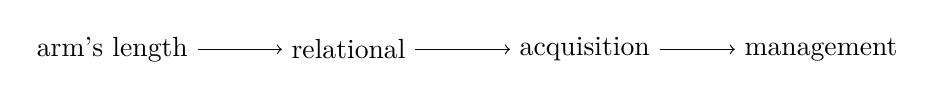
\begin{tikzpicture}
\node (a) at (0,0) {arm's length};
\node (b) at (3,0) {relational};
\node (c) at (6,0) {acquisition};
\node (d) at (9,0) {management};
\graph { (a) -> (b) -> (c) -> (d)};
\end{tikzpicture}
\end{frame}

\begin{frame}{This paper}
\protect\hypertarget{this-paper}{}
\begin{itemize}
\tightlist
\item
  Compile new data on which firm is run by which manager: Hungary,
  1980--2018.
\item
  Measure different degrees of foreign control:

  \begin{enumerate}
  \tightlist
  \item
    acquisition
  \item
    replace CEO
  \item
    hire expat CEO
  \end{enumerate}
\item
  Results:

  \begin{itemize}
  \tightlist
  \item
    Exporters and low-productivity firms become more tightly controlled.
  \item
    Firms with high intangible capital receive local managers.
  \item
    Expat controlled firms become more productive and more likely to
    export (relative to other forms of control).
  \end{itemize}
\end{itemize}
\end{frame}

\hypertarget{data}{%
\section{Data}\label{data}}

\begin{frame}{Data}
\begin{block}{Hungarian Manager Database}
\protect\hypertarget{hungarian-manager-database}{}
\begin{itemize}
\tightlist
\item
  coverage: universe of corporations, 1980--2018
\item
  CEO: highest officer of corporation as specified in corporate law.

  \begin{itemize}
  \tightlist
  \item
    information: name, mother's name, address, tenure at firm
  \end{itemize}
\item
  1 million firms, 2 million CEOs, 5 million job spells
\end{itemize}
\end{block}

\begin{block}{Balance sheet data}
\protect\hypertarget{balance-sheet-data}{}
\begin{itemize}
\tightlist
\item
  coverage: universe of double entry firms, 1980--2018
\item
  information: sales, exports, employment, equipment, immaterials etc.
\end{itemize}
\end{block}

\begin{block}{Customs statistics}
\protect\hypertarget{customs-statistics}{}
\begin{itemize}
\tightlist
\item
  coverage: universe of direct exports and imports, 1992--2003
\item
  information: product code, partner country, firm id, value
\end{itemize}
\end{block}
\end{frame}

\begin{frame}{Names}
\protect\hypertarget{names}{}
\begin{itemize}
\tightlist
\item
  We use manager names to infer

  \begin{enumerate}
  \tightlist
  \item
    CEO change
  \item
    nationality
  \item
    gender (not used today)
  \end{enumerate}
\item
  Foreign manager: firm representative with a non-Hungarian first name

  \begin{enumerate}
  \tightlist
  \item
    e.g.~Eva Bauer v Bauer Éva
  \item
    but: George Soros v Soros György
  \end{enumerate}
\item
  Allow for misspelling, omitted middle name, missing data (jr, dr)
\end{itemize}
\end{frame}

\begin{frame}{Sample}
\protect\hypertarget{sample}{}
\begin{itemize}
\tightlist
\item
  Exclude:

  \begin{itemize}
  \tightlist
  \item
    employing less than 20 people
  \item
    financial sector
  \item
    domestic firms with expat CEO
  \item
    greenfield FDI
  \item
    firms with more than 15 CEOs
  \end{itemize}
\item
  Left with 24,500 firms
\end{itemize}
\end{frame}

\begin{frame}{Largest investment partners of Hungary 1992--2003}
\protect\hypertarget{largest-investment-partners-of-hungary-19922003}{}
\includegraphics{figure/map.png}
\end{frame}

\begin{frame}{Foreign owners often replace managers}
\protect\hypertarget{foreign-owners-often-replace-managers}{}
\includegraphics{figure/sample-size.png}
\end{frame}

\hypertarget{estimation}{%
\section{Estimation}\label{estimation}}

\begin{frame}{Estimating equations}
\protect\hypertarget{estimating-equations}{}
\begin{block}{Selection}
\protect\hypertarget{selection}{}
Sample: 1 year before acquisition \[
\Pr(\text{CONTROL}_{it}=k) = \Lambda(\mu_{st} + \gamma X_{it})
\] estimated with multinomial or ordered logit
\end{block}

\begin{block}{Diff-in-diff (!)}
\protect\hypertarget{diff-in-diff}{}
Sample: acquisitions \[
Y_{ist} = \alpha_i + \mu_{st} + \sum_{k=1}^3 \beta_k \text{CONTROL}_{it}^k + u_{ist}
\]
\end{block}
\end{frame}

\begin{frame}{Positive selection on capital and exports, negative on
TFP}
\protect\hypertarget{positive-selection-on-capital-and-exports-negative-on-tfp}{}
\input{table/selection.tex}
\end{frame}

\hypertarget{differences-in-differences}{%
\section{Differences in differences}\label{differences-in-differences}}

\begin{frame}{Differences in differences}
\protect\hypertarget{differences-in-differences-1}{}
\[
Y_{it} = \alpha_i + \nu_t + \beta \text{CONTROL}_{it} + u_{it}
\]

\begin{block}{Old diff-in-diff}
\protect\hypertarget{old-diff-in-diff}{}
Estimate by two-way fixed effects.
\end{block}

\begin{block}{New diff-in-diff}
\protect\hypertarget{new-diff-in-diff}{}
Compute group-specific treatment effects and aggregate. (Callaway and
Sant'Anna 2020)
\end{block}
\end{frame}

\begin{frame}{Problem with TWFE}
\protect\hypertarget{problem-with-twfe}{}
Model may be misspecified. Often, \(\beta\) is heterogeneous or
increases over treatment length.

This is a problem if treatment is staggered, especially in long panel
(our case).

Long treated firms will act as a control, biasing \(\hat\beta\). May
even have different sign than all the individual treatment effects.
\end{frame}

\begin{frame}{Callaway - Sant'Anna solution}
\protect\hypertarget{callaway---santanna-solution}{}
\(G_{i}\): time of treatment of unit \(i\) (may be \(\infty\))

\(C_{gt} = \{i: G_i > \max(g,t)\}\): control group is not yet treated

\[
\gamma_{gt} := E_{i: G_i=g} (Y_{it} - Y_{ig})
- E_{i\in C_{gt}} (Y_{it} - Y_{ig})
\]

Aggregate \(\gamma_{gt}\) with ``suitable'' weights
\end{frame}

\begin{frame}{Multiple treatments}
\protect\hypertarget{multiple-treatments}{}
We have three treatments: acquisition only, domestic hire, expat hire.

How to do Callaway-Sant'Anna in this case?

Make sure treatments don't ``leak'' into controls.
\end{frame}

\begin{frame}{Our solution}
\protect\hypertarget{our-solution}{}
\(G_{i}^k\): time of treatment \(k\) of unit \(i\) (may be \(\infty\))

\(C_{gt} = \{i: \min_k G_i^k > \max(g,t)\}\): control group is not yet
treated with \textbf{any} of the treatments

\[
\gamma_{gt}^k := E_{i: G_i=g} (Y_{it} - Y_{ig})
- E_{i\in C_{gt}} (Y_{it} - Y_{ig})
\]

Each treatment has the \textbf{same} control group.

We also do inverse-probability weighting within control group (Abadie
2005). This helps kill pretrends.
\end{frame}

\hypertarget{results}{%
\section{Results}\label{results}}

\hypertarget{without-change-in-management}{%
\section{Without change in
management}\label{without-change-in-management}}

\begin{frame}{No effects of foreign acquisition on employment}
\protect\hypertarget{no-effects-of-foreign-acquisition-on-employment}{}
\includegraphics{figure/event_study/no_hire_lnL.png}
\end{frame}

\begin{frame}{No effects of foreign acquisition on capital}
\protect\hypertarget{no-effects-of-foreign-acquisition-on-capital}{}
\includegraphics{figure/event_study/no_hire_lnK.png}
\end{frame}

\begin{frame}{No effects of foreign acquisition on labor productivity}
\protect\hypertarget{no-effects-of-foreign-acquisition-on-labor-productivity}{}
\includegraphics{figure/event_study/no_hire_lnQL.png}
\end{frame}

\begin{frame}{\ldots or TFP}
\protect\hypertarget{or-tfp}{}
\includegraphics{figure/event_study/no_hire_TFP_cd.png}
\end{frame}

\begin{frame}{Some transitory increase in exporting}
\protect\hypertarget{some-transitory-increase-in-exporting}{}
\includegraphics{figure/event_study/no_hire_exporter.png}
\end{frame}

\hypertarget{hire-a-local-manager}{%
\section{Hire a local manager}\label{hire-a-local-manager}}

\begin{frame}{Fast productivity growth after local manager is hired}
\protect\hypertarget{fast-productivity-growth-after-local-manager-is-hired}{}
\includegraphics{figure/event_study/local_hire_lnQL.png}
\end{frame}

\begin{frame}{Also in TFP}
\protect\hypertarget{also-in-tfp}{}
\includegraphics{figure/event_study/local_hire_TFP_cd.png}
\end{frame}

\hypertarget{hire-an-expat-manager}{%
\section{Hire an expat manager}\label{hire-an-expat-manager}}

\begin{frame}{Fast employment growth after expat manager is hired}
\protect\hypertarget{fast-employment-growth-after-expat-manager-is-hired}{}
\includegraphics{figure/event_study/expat_hire_lnL.png}
\end{frame}

\begin{frame}{Positive capital investments after expat manager is hired}
\protect\hypertarget{positive-capital-investments-after-expat-manager-is-hired}{}
\includegraphics{figure/event_study/expat_hire_lnK.png}
\end{frame}

\begin{frame}{Productivity growth of same magnitude as with local
manager}
\protect\hypertarget{productivity-growth-of-same-magnitude-as-with-local-manager}{}
\includegraphics{figure/event_study/expat_hire_lnQL.png}
\end{frame}

\begin{frame}{Also in TFP}
\protect\hypertarget{also-in-tfp-1}{}
\includegraphics{figure/event_study/expat_hire_TFP_cd.png}
\end{frame}

\begin{frame}{Large effects on exporting}
\protect\hypertarget{large-effects-on-exporting}{}
\includegraphics{figure/event_study/expat_hire_exporter.png}
\end{frame}

\hypertarget{market-access}{%
\section{Market access}\label{market-access}}

\begin{frame}{Market access}
\protect\hypertarget{market-access-1}{}
Ongoing work with Krisztina Orbán and Álmos Telegdy.
\end{frame}

\begin{frame}{Infer nationality from name}
\protect\hypertarget{infer-nationality-from-name}{}
\begin{tabular}{llcc|ccc}
Addr. & Name & Nat. & Lang. & AT & DE & IT\\
\hline
DE & Klaudia Wolf & de & de         & N+L & A+N+L & \\
AT & Enrico Mazzanti & it & de,it   & A+L & L & N+L\\
IT & Fioretta Luchesi & it & it     & & & A+N+L
\end{tabular}
\end{frame}

\begin{frame}{Estimating equation}
\protect\hypertarget{estimating-equation}{}
For each firm-year, take 24 major partner countries. What is the
probability to export/import to/from that country, \emph{relative to all
other countries}?

\[
\Pr(X_{ict}=1) = 
\mu_{ct} + \nu_{it} 
\] \[
{}+ \beta_1 \text{ADDRESS}_{ict} 
{}+ \beta_2 \text{NATIONALITY}_{ict} 
{}+ \beta_3 \text{LANGUAGE}_{ict} 
{}+ u_{ict}
\]
\end{frame}

\begin{frame}{Manager address and nationality matter for trade}
\protect\hypertarget{manager-address-and-nationality-matter-for-trade}{}
\begin{tabular}{lcccc} \hline
& (1) & (2) & (3) & (4) \\
& export & export & import & import \\ \hline
&  &  &  &  \\
ADDRESS & 0.142*** & 0.100*** & 0.220*** & 0.183*** \\
& (0.031) & (0.031) & (0.038) & (0.040) \\
NATIONALITY & 0.037** & 0.034* & 0.091*** & 0.090*** \\
& (0.018) & (0.018) & (0.026) & (0.025) \\
LANGUAGE & -0.025** & -0.032*** & 0.005 & 0.003 \\
& (0.011) & (0.012) & (0.012) & (0.012) \\
ADDRESS (owner) &  & 0.090*** &  & 0.075*** \\
&  & (0.021) &  & (0.021) \\
LANGUAGE (owner) &  & 0.018** &  & 0.005 \\
&  & (0.009) &  & (0.010) \\
&  &  &  &  \\
Observations & 67,965 & 67,965 & 64,834 & 64,834 \\
R-squared & 0.232 & 0.235 & 0.269 & 0.270 \\
Mean dep.~var.& 0.0387 & 0.0387 & 0.0624 & 0.0624 \\ \hline
\end{tabular}
\end{frame}

\hypertarget{discussion}{%
\section{Discussion}\label{discussion}}

\begin{frame}{Effects are large}
\protect\hypertarget{effects-are-large}{}
\begin{block}{Fixed-cost estimates in Halpern, Koren and Szeidl (2015)}
\protect\hypertarget{fixed-cost-estimates-in-halpern-koren-and-szeidl-2015}{}
Equivalent to \$12-14,000 drop in fixed costs `'per year''.

\begin{tabular}{l|cc}
Scenario & Import hazard & Fixed cost \\
\hline
Average firm & 0.010 & \$15,000\\
Only owner & 0.081 & \$2,300\\
Only manager & 0.106 & \$1,700\\
Both & 0.226 & \$600
\end{tabular}
\end{block}

\begin{block}{Trade experience premia}
\protect\hypertarget{trade-experience-premia}{}
Mion, Opromolla and Sforza (2016) estimate a 0.01--0.04 increase in
hazard after manager with relevant export experience joins. Bisztray,
Koren and Szeidl (2018) estimiate 0.002--0.005 peer effects in
importing.
\end{block}
\end{frame}

\begin{frame}{Summary}
\protect\hypertarget{summary}{}
\begin{enumerate}
\tightlist
\item
  Acquired firms only change business practices if management is also
  changed.
\item
  It matters who the managers are where they come from.
\item
  Managers matter more than owners for firm performance.
\end{enumerate}
\end{frame}

\begin{frame}{Two directions}
\protect\hypertarget{two-directions}{}
\begin{enumerate}
\tightlist
\item
  Causes: incomplete contracts, loyalty, embodied knowledge.
\item
  Consequences: inelastic supply of good management, interesting
  reallocation of managers across firms.
\end{enumerate}
\end{frame}

\hypertarget{a-potential-model}{%
\section{A potential model}\label{a-potential-model}}

\begin{frame}{Production function}
\protect\hypertarget{production-function}{}
Firm \(j\), market \(i\) \[
Q_{ij}=A_j K_{ij}^\alpha L_{ij}^{1-\alpha}\text{ with } i=H,F
\] in contrast to \[
\sum_iQ_{ij} = A_jK_j^\alpha L_j^{1-\alpha}
\] Firm characterized by \((A_j, K_{Hj}, K_{Fj})\)
\end{frame}

\begin{frame}{Market access skills}
\protect\hypertarget{market-access-skills}{}
Manager \(m\), market \(i\) \[
\kappa_{im}p_i \text{ with }\kappa_{im} \in (0,1)
\] Manager characterized by \((\kappa_{Hm}, \kappa_{Fm})\)
\end{frame}

\begin{frame}{Net revenue per market}
\protect\hypertarget{net-revenue-per-market}{}
\[
\kappa_{im}p_i A_j K_{ij}^{\alpha} L_{ij}^{1-\alpha} - w L_{ij}
\] Labor frictionlessly hired, \[
R_{ijm} =  \left(\frac {1-\alpha} {w}\right)^{1/\alpha-1} 
{(\kappa_{im}p_i)^{1/\alpha}\strut} {A_j^{1/\alpha} K_{ij}\strut}
\] \[
R_{ijm} = \tilde \kappa_{im} \tilde K_{ij}
\]
\end{frame}

\begin{frame}{Assignment}
\protect\hypertarget{assignment}{}
Firms hire managers in frictionless, competitive markets. Optimal
manager maximizes net revenue minus her wage, \[
\max_m \alpha\sum_i R_{ijm} - \nu_m =  \max_m \alpha\sum_i \tilde\kappa_{im}\tilde K_{ij} - \nu_m,
\]
\end{frame}

\begin{frame}{Equilibrium}
\protect\hypertarget{equilibrium}{}
Given fixed distributions over \((A_j, K_{Hj}, K_{Fj})\) and
\((\kappa_{Hm}, \kappa_{Fm})\) (with \(\#j = \#m\)), determine

\begin{itemize}
\tightlist
\item
  firm-manager assignment: \(\mu(j,m)\)
\item
  manager wages: \(\nu_m\)
\item
  firm profits: \(\pi_j\)
\item
  revenue per market: \(R_{ijm}\)
\end{itemize}
\end{frame}

\begin{frame}{Key ingredients}
\protect\hypertarget{key-ingredients}{}
\begin{enumerate}
\tightlist
\item
  Diminishing returns within each market
\item
  Inelastic supply of manager skills
\item
  Complementarity of manager skills with firm capital
\end{enumerate}
\end{frame}

\begin{frame}{Optimal transport}
\protect\hypertarget{optimal-transport}{}
Equilibrium assingment is equivalent to following optimal transport
problem (Galichon 2016) \[
\int_{j,m}\mu(j,m) (\tilde {\mathbf K}_j - \tilde{\mathbf\kappa}_m)^2 djdm \to \min
\] s.t. \[
\int_j \mu(j,m) dj = \mu(j)
\] \[
\int_m \mu(j,m) dm = \mu(m)
\] Focus on discrete manager types, continuous firm types.
\end{frame}

\hypertarget{predictions}{%
\section{Predictions}\label{predictions}}

\begin{frame}{Cross sectional predictions}
\protect\hypertarget{cross-sectional-predictions}{}
\begin{enumerate}
\tightlist
\item
  Conditional on \(R_{j}\), there is heterogeneity in \(R_{Fj}/R_{Dj}\).
\item
  Managers at larger firms earn more.
\item
  Manager wages convex in \(\mathbf K\).
\item
  Conditional on \(R_{Dj}\), managers at high \(R_{Fj}\) firms earn
  more.
\end{enumerate}
\end{frame}

\begin{frame}{Export heterogeneity}
\protect\hypertarget{export-heterogeneity}{}
\[
\text{Var}\ln R_{ij} =
    \text{Var}\ln \tilde \kappa_{im} +
    \text{Var}\ln \tilde K_{jm} +
    2\text{Cov}(\ln \tilde \kappa_{im},
                \ln \tilde K_{jm})
\]

\begin{itemize}
\tightlist
\item
  additional heterogeneity in managers:
  \(\text{Var}\ln \tilde \kappa_{im}>0\)
\item
  complementarity of managers and firms:
  \(2\text{Cov}(\ln \tilde \kappa_{im},\ln \tilde K_{jm})>0\)
\end{itemize}
\end{frame}

\hypertarget{comparative-statics}{%
\section{Comparative statics}\label{comparative-statics}}

\begin{frame}{Supply shock}
\protect\hypertarget{supply-shock}{}
\end{frame}

\begin{frame}{Trade liberalization}
\protect\hypertarget{trade-liberalization}{}
Export markets become liberalized (\(p_F\) increases).

\begin{enumerate}
\tightlist
\item
  Managers with export skills earn more.
\item
  Net entry into exporting is zero (by assumption).
\item
  Export-skilled managers move from low export-intensity firms to high
  export-intensity firms. (magnifying export heterogeneity)
\end{enumerate}
\end{frame}

\begin{frame}{Firms run by expat managers dominate local firms in MLR
sense}
\protect\hypertarget{firms-run-by-expat-managers-dominate-local-firms-in-mlr-sense}{}
\includegraphics[width=\textwidth,height=0.7\textheight]{figure/FSD.pdf}
\end{frame}

\begin{frame}{CEO wages at large firms have increased
disproportionately}
\protect\hypertarget{ceo-wages-at-large-firms-have-increased-disproportionately}{}
\includegraphics[width=\textwidth,height=0.7\textheight]{figure/wage_premium.pdf}
\end{frame}

\begin{frame}{Wage returns to exporting increased among CEOs}
\protect\hypertarget{wage-returns-to-exporting-increased-among-ceos}{}
\includegraphics[width=\textwidth,height=0.7\textheight]{figure/exporter_wage_premium.png}
\end{frame}

\hypertarget{conclusions}{%
\section{Conclusions}\label{conclusions}}

\begin{frame}{Conclusions}
\protect\hypertarget{conclusions-1}{}
\begin{itemize}
\tightlist
\item
  What are the causes and consequences of foreign acquisitions?
\item
  We ask when managers are also replaced.
\item
  Using data on the universe of foreign acquisitions in Hungary,
  1980-2018, we estimate that exporters and low-productivity firms
  become more tightly controlled.
\item
  Foreign controlled firms become more productive and more likely to
  export.
\item
  These facts help inform theories about the boundaries of global firms
  and about the role of managers in firm performance.
\end{itemize}
\end{frame}

\end{document}
